%{{{ Preamble

\documentclass{article}
\usepackage{graphicx}
\graphicspath{{./}{../FIGs/}{../Logos/}}
\ifx\HCode\Undef
\DeclareGraphicsExtensions{.pdf,.png}
\else
\usepackage{tex4ht}
\DeclareGraphicsExtensions{.svg, .png, .jpg}
\fi
\usepackage{hyperref}
\usepackage{color}

\usepackage{amsmath}

%\renewcommand{\rmdefault}{ptm}
%\renewcommand\familydefault{\sfdefault}

%}}}

%{{{ Front

\author{%
Crist\'obal Medina L\'opez, Juan Pablo Garc\'ia Ortiz and Juan Alvaro Mu\~noz Naranjo,\\\href{http://www.luxunda.es/}{Luxunda SL}. \\
~\\
Leocadio Gonz\'alez Casado and Vicente Gonz\'alez Ruiz,\\\href{http://www.hpca.ual.es/}{SAL, UAL}.
}

\newcommand{\thankss}{
%{{{

  \vbox{
    \ifx \HCode\Undfef
    \else
    \HCode{<div style="text-align:center;">
      <img width=800 src="FIGs/thanks.svg" align="top"/>
      </div>
    }
    \fi
  }

%}}}
}

\title{Live-Video Streaming over Internet using P2PSP}
\date{Jun 17, 2015 \\~\\ \url{http://slides.p2psp.org/2015-06-Barcelona} \\~\\ \thankss}

%}}}

\begin{document}
%{{{ Body

%{{{ Definitions

% Family       Font Name
% pag          Avant Garde *
% fvs          Bitstream Vera Sans
% pbk          Bookman
% bch          Charter
% ccr          Computer Concrete
% cmr          Computer Modern
% pcr          Courier
% mdugm        Garamond
% phv          Helvetica *
% fi4          Inconsolata
% lmr          Latin Modern
% LinuxBiolinumT-OsF     Linux Biolinum (formerly 'fxb' in older package versions)
% LinuxLibertineT-OsF    Linux Libertine (formerly 'fxl' in older package versions)
% pnc          New Century Schoolbook
% ppl          Palatino
% ptm          Times
% uncl         Uncial
% put          Utopia
% pzc          Zapf Chancery

%\fontfamily{pag}\selectfont
\fontfamily{phv}\selectfont
%\sffamily
%\def\normalfont{\sffamily}
%\renewcommand{\familydefault}{cmss} \
%\renewcommand{\familydefault}{\sfdefault}
%\selectfont

%}}}

\maketitle

~\\
~\\
~\\

\section{\href{http://www.p2psp.org/en/}{P2PSP (Peer-to-Peer ``Straightforward'' Protocol)}}
%{{{

\begin{itemize}
\item \emph{Definition:} An application-layer protocol for the real-time streaming of media
  content between networked entities.
\item \emph{Topology:} Push-based fully-connected mesh overlay.
\ifx \HCode\Undfef
%\begin{center}
%  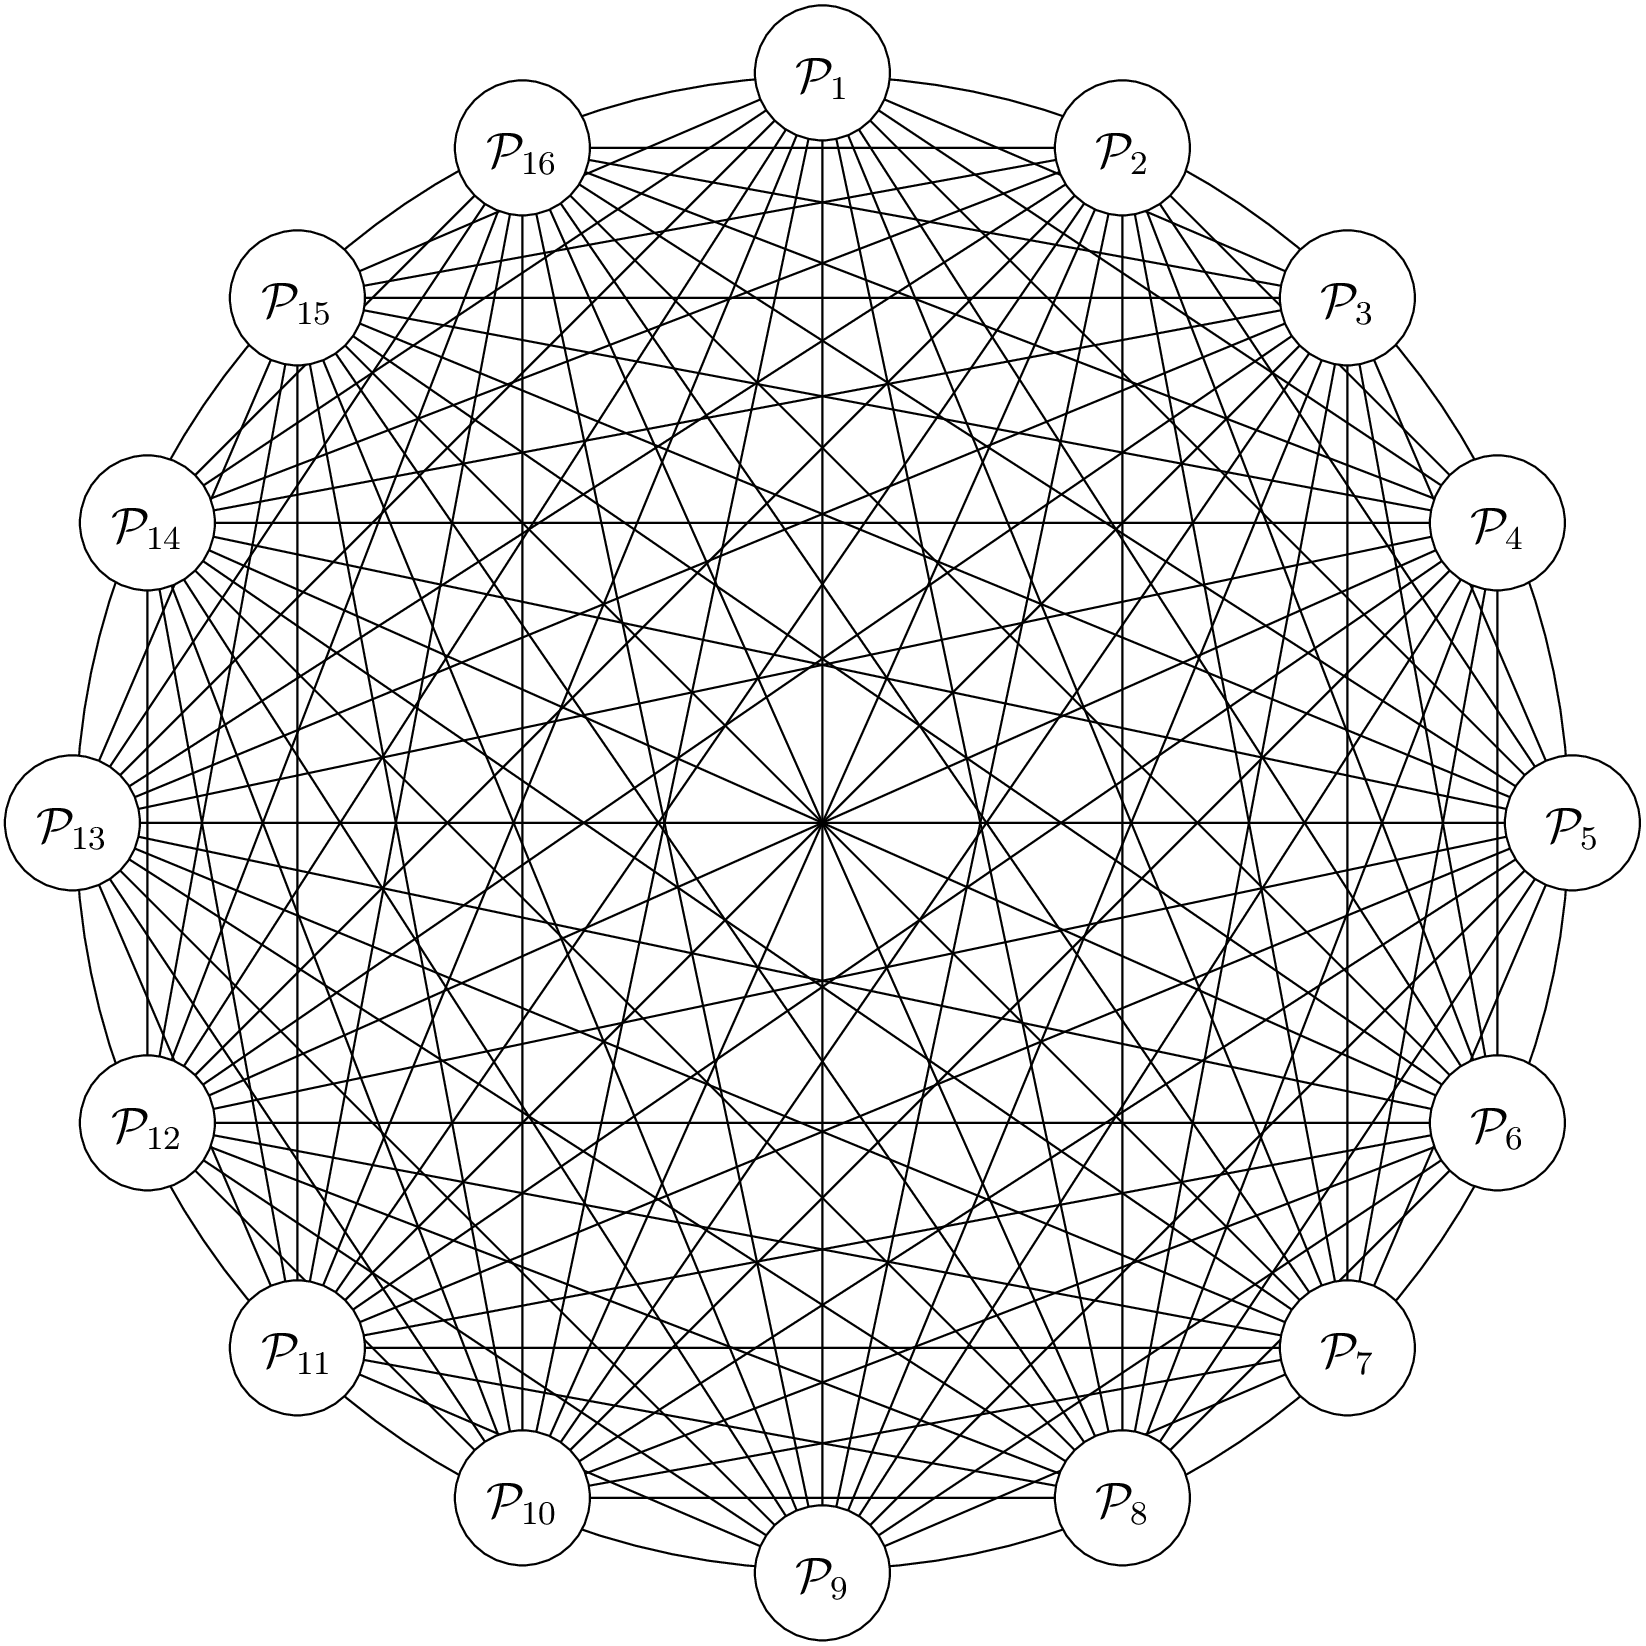
\includegraphics[width=1.0\textwidth]{FIGs/full-mesh}
%\end{center}
\else
\HCode{
  <div style="text-align:center;">
    <img height="600" src="FIGs/full-mesh.svg" />
  </div>
}
\fi

\item \emph{Proposal:} Emulate the IP multicast functionality as close as possible.
\item \emph{Availability:} An
  \href{https://www.gnu.org/copyleft/gpl.html}{open-source}
  implementation is downloadable from
  \href{https://github.com/p2psp}{GitHub}.
\item \emph{Support:} P2PSP is being developed with the financial
  support of the Spanish Ministry of Economy and Competitiveness
  (TIN2012-37483-C03-03) and Junta de Andaluc\'{\i}a (P10-TIC-6548),
  the European Regional Development Fund (ERDF), Campus de Excelencia
  Internacional Agroalimentario (ceiA3) and
  \href{http://www.google-melange.com/gsoc/org/list/public/google/gsoc2015}{Google
    Summer of Code 2015}.
\end{itemize}

%}}}

\section{\href{https://en.wikipedia.org/wiki/IPTV}{IP-TV} over P2PSP}
%{{{

\ifx \HCode\Undfef
%\begin{center}
%  \includegraphics[width=1.0\textwidth]{spain-IPTV-P2P}
%\end{center}
\else
\HCode{
  <div style="text-align:center;">
    <img height="600" src="http://slides.p2psp.org/2014-11-Jornada-Contenidos-Digitales-UAL/FIGs/spain-IPTV-P2P.svg" />
  </div>
}
\fi

%}}}

\section{Designed as a collection of Sets of Rules}
%{{{

\begin{itemize}
\item Each Set of Rules addresses a specific situation.
\end{itemize}

\begin{center}
\begin{verbatim}
                  +-----+
                  | EMS |
                  +-----+
                  | NTS |
 +-----+-----+    +-----+-----+-----+-----+-----+-----+
 | DPS | MCS |    | FNS | ACS | LRS | CIS | DPS | MCS |
 +-----+-----+----+-----+-----+-----+-----+-----+-----+
 |      IMS       |                DBS                |
 +----------------+-----------------------------------+
 |  IP multicast  |             IP (unicast)          |
 +----------------+-----------------------------------+
\end{verbatim}
\end{center}

%}}}

\section{\href{http://www.p2psp.org/en/p2psp-protocol?cap=indexsu4.xht\#x11-90004.4}{IP Mulicast Set (IMS) of Rules}}
%{{{

\begin{itemize}
\item \emph{Context of use:} IP multicast is available.
\item \emph{Clue:} A splitter sends chunks to peers using an IP multicast channel
  and therefore, peers do not need to communicate each other.
\item \emph{Functionality:} Provides a buffering technique to hidden the (physical) network jitter.
\end{itemize}
\ifx \HCode\Undfef
%\begin{center}
%  \includegraphics[width=0.5\textwidth]{multicast-splitter}
%\end{center}
\else
\HCode{
  <div style="text-align:center;">
    <img height="500" src="http://slides.p2psp.org/2014-11-Jornada-Contenidos-Digitales-UAL/FIGs/multicast-splitter.svg" />
  </div>
}
\fi

%}}}

\section{\href{http://www.p2psp.org/en/p2psp-protocol?cap=indexsu5.xht\#x12-100004.5}{Data Broadcasting Set (DBS) of Rules}}
%{{{

\begin{itemize}
\item \emph{Context of use:} IP multicast is NOT available.
\item \emph{Clue:} The splitter uses a Round-Robing broadcasting
  strategy and Unicast comunications. Peers shares every chunk
  received from the splitter.
\end{itemize}

\ifx \HCode\Undfef
%\begin{center}
%  \includegraphics[width=0.5\textwidth]{congestion_control2}
%\end{center}
\else
\HCode{
  <div style="text-align:center;">
    <img height="500" src="http://slides.p2psp.org/2015-01-Elche/FIGs/congestion_control2.svg" />
  </div>
}
\fi

%}}}

\section*{\href{https://en.wikipedia.org/wiki/Network_address_translation}{NAT: Network Address Translation}}
%{{{

\ifx \HCode\Undfef
%\begin{center}
%  \includegraphics[width=0.5\textwidth]{NATting}
%\end{center}
\else
\HCode{
  <div style="text-align:center;">
    <img height="400" src="http://slides.p2psp.org/2015-01-Elche/FIGs/NATting.svg" />
  </div>
}
\fi

%}}}

\section{Full-cone Nat Set (FNS) of Rules}
%{{{

\begin{itemize}
\item \emph{Context of use:} In those peers that run behind a full-cone NAT.
\item \emph{Clue:} To enable inbound UDP traffic from the splitter to
  the incomming the peer, this sends a [hello] message to the splitter. 
\end{itemize}

\ifx \HCode\Undfef
%\begin{center}
%  \includegraphics[width=0.5\textwidth]{IMS_DBS_FNS_timeline}
%\end{center}
\else
\HCode{
  <div style="text-align:center;">
    <img height="400" src="http://slides.p2psp.org/2015-01-Elche/FIGs/IMS_DBS_FNS_timeline.svg" />
  </div>
}
\fi

%}}}

\section{\href{http://www.p2psp.org/en/p2psp-protocol?cap=indexsu6.xht\#x14-110004.6}{Adaptive Chunk-rate Set (ACS) of Rules}}
%{{{

\begin{itemize}
\item \emph{Context of use:} Users allow the existence of unsupportive peers.
\item \emph{Clue:} For every peer, the splitter gathers statistics
  from the monitor(s) peer(s) about the lost chunk ratio and estimates
  a capacity.
\end{itemize}

\ifx \HCode\Undfef
%\begin{center}
%  \includegraphics[width=0.5\textwidth]{}
%\end{center}
\else
\HCode{
  <div style="text-align:center;">
    <img height="400" src="http://slides.p2psp.org/2014-11-Jornada-Contenidos-Digitales-UAL/FIGs/ACS.svg" />
  </div>
}
\fi

%}}}

\section{\href{http://www.p2psp.org/en/p2psp-protocol?cap=indexsu7.xht\#x15-120004.7}{Lost chunks Recovery Set (LRS) of Rules}}
%{{{

\begin{itemize}
\item \emph{Context of use:} The splitter can lost some chunks.
\item \emph{Clue:} Massively lost chunks (those that have not arrived
  to none of the monitor peers) are re-sent by the splitter (usually
  to one or more monitor peers).
\end{itemize}

\ifx \HCode\Undfef
%\begin{center}
%  \includegraphics[width=0.5\textwidth]{LRS}
%\end{center}
\else
\HCode{
  <div style="text-align:center;">
    <img height="400" src="http://slides.p2psp.org/2014-11-Jornada-Contenidos-Digitales-UAL/FIGs/LRS.svg" />
  </div>
}
\fi

%}}}

\section{\href{http://www.p2psp.org/en/p2psp-protocol?cap=indexsu12.xht\#x20-170004.12}{End-point Masquerading Set (EMS) of Rules}}
%{{{

\begin{itemize}
\item \emph{Context of use:} Two or more peers are in the same private network.
\item \emph{Clue:} These peers should use their private addresses to
  communicate between them but their public end-points to communicate
  with other peers.
\end{itemize}

\ifx \HCode\Undfef
%\begin{center}
%  \includegraphics[width=0.5\textwidth]{EMS}
%\end{center}
\else
\HCode{
  <div style="text-align:center;">
    <img height="300" src="http://slides.p2psp.org/2014-11-Jornada-Contenidos-Digitales-UAL/FIGs/EMS.svg" />
  </div>
}
\fi

%}}}

\section*{\href{http://en.wikipedia.org/wiki/Network_address_translation}{Full-cone NATs versus Restricted-cone NATs}}
%{{{

\ifx \HCode\Undfef
%\begin{center}
%  \includegraphics[width=0.5\textwidth]{full-cone-NAT}
%  \includegraphics[width=0.5\textwidth]{restricted-cone-NAT}
%\end{center}
\else
\HCode{
  <div style="text-align:center;">
    <img height="600" src="http://slides.p2psp.org/2015-01-Elche/FIGs/full-cone-NAT.svg" />
    <img height="600" src="http://slides.p2psp.org/2015-01-Elche/FIGs/restricted-cone-NAT.svg" />
  </div>
}
\fi

%}}}

\section{\href{http://www.p2psp.org/en/p2psp-protocol?cap=indexsu9.xht\#x18-140004.9}{Restricted (-Cone) NAT Traversal Set (RTS) of Rules}}
%{{{

\begin{itemize}
\item \emph{Context of use:} Peers are behind cone and restricted-cone NATs.
\item \emph{Clue:} All NATted peers of the team send to the incomming
  peer $P_{i+1}$ a [hello] message to create an entry in their NATs
  that enables the incomming traffic from $P_{i+1}$.
\end{itemize}

\ifx \HCode\Undfef
%\begin{center}
%  \includegraphics[width=0.5\textwidth]{RTS}
%\end{center}
\else
\HCode{
  <div style="text-align:center;">
    <img height="500" src="FIGs/RTS.svg" />
  </div>
}
\fi

%}}}

\section*{\href{http://en.wikipedia.org/wiki/Network_address_translation}{Cone NATs versus Symmetric NATs}}
%{{{

\ifx \HCode\Undfef
%\begin{center}
%  \includegraphics[width=0.5\textwidth]{cone-NAT}
%  \includegraphics[width=0.5\textwidth]{symmetric-NAT}
%\end{center}
\else
\HCode{
  <div style="text-align:center;">
    <img height="300" src="http://slides.p2psp.org/2015-01-Elche/FIGs/cone-NAT.svg" />
    <img height="300" src="http://slides.p2psp.org/2015-01-Elche/FIGs/symmetric-NAT.svg" />
  </div>
}
\fi

%}}}

\section{\href{http://www.p2psp.org/en/p2psp-protocol?cap=indexsu9.xht\#x18-140004.9}{Symmetric NAT Traversal Set (STS) of Rules}}
%{{{

\begin{itemize}
\item \emph{Context of use:} Peers are behind symmetric NATs.
\item \emph{Clue:} NATted peers must use some prediction technique to
  find out which public port will use the NATs of the other
  peers. Unfortunately NAT behaviours are not standarized an this is
  an open problem :-/
\end{itemize}

\ifx \HCode\Undfef
%\begin{center}
%  \includegraphics[width=0.5\textwidth]{STS}
%\end{center}
\else
\HCode{
  <div style="text-align:center;">
    <img height="1000" src="FIGs/STS.svg" />
  </div>
}
\fi

%}}}

\section{\href{http://www.p2psp.org/en/p2psp-protocol?cap=indexsu11.xht\#x20-160004.11}{Content Integrity Set (CIS)}}
%{{{

\begin{itemize}
\item \emph{Context of use:} One or more malicious peers want to
  poison the stream.
\item \emph{Clues:} The splitter should identify them and stop sending
  more chunks.
  \begin{enumerate}
  \item Security level 1: Trusted peers send to the splitter a hash of
    each chunk and the splitter checks if the chunks have been
    poisoned.
    \item Security level 2: Chunks are digitally signed (to allow
      peers to know if their are been attacked) and the splitter
      gathers statistics from all peers of the team.
  \end{enumerate}
\end{itemize}

%}}}

\section{\href{http://www.p2psp.org/en/p2psp-protocol?cap=indexsu12.xht\#x21-180004.12}{Data Privacy Set (DPS)}}
%{{{

\begin{itemize}
\item \emph{Context of use:} Pay-per-view services, high-privacy multicasting.
\item \emph{Clues:}
    \begin{enumerate}
  \item Security level 1: Media is encripted in the source and the
    licit players know the description keys (splitter and peers are
    oblivious to this process).
    \item Security level 2: The splitter controls who can join the
      team.
  \end{enumerate}
\end{itemize}

%}}}

\section{\href{http://www.p2psp.org/en/p2psp-protocol?cap=indexsu11.xht\#x20-160004.11}{Multi-Channel Set (MCS)}}
%{{{

\begin{itemize}
\item \emph{Context of use:} Concurrent channel streaming, 3D video streaming, etc.
\item \emph{Clues:}
  \begin{enumerate}
  \item User run several peers concurrently.
  \item Each peers belong to a different team (channel).
  \item Traffic should be prioritized.
  \end{enumerate}
\end{itemize}
    
\ifx \HCode\Undfef
%\begin{center}
%  \includegraphics[width=0.5\textwidth]{3d-example}
%\end{center}
\else
\HCode{
  <div style="text-align:center;">
    <img height="500" src="http://slides.p2psp.org/2014-11-Jornada-Contenidos-Digitales-UAL/FIGs/3d-example.svg" />
  </div>
}
\fi

%}}}

\part*{}
%{{{

\begin{center}
~\\ ~\\ ~\\ \Huge{Thanks!}~\\ ~\\ ~\\ ~\\
\end{center}

%}}}

%}}}
\end{document}
